\documentclass{article}

\usepackage{graphicx}
\usepackage{subfigure}
\usepackage[hypcap]{caption}
\usepackage{listings}
\usepackage{float}
\floatstyle{plaintop}
\restylefloat{table}

\title{Experimental Design and Data Analysis: Assignment 5}
\author{Andrew Bedard(2566978) \& Simone van Gompel(2567525) \\ Group 19}

\begin{document}

  \maketitle

  \section*{Exercise 1}
    \subsection*{1}
    \subsection*{2}
    \subsection*{3}
    \subsection*{4}
    
  \section*{Exercise 2}
    \subsection*{1}
      \begin{figure}[H]
          \centering
          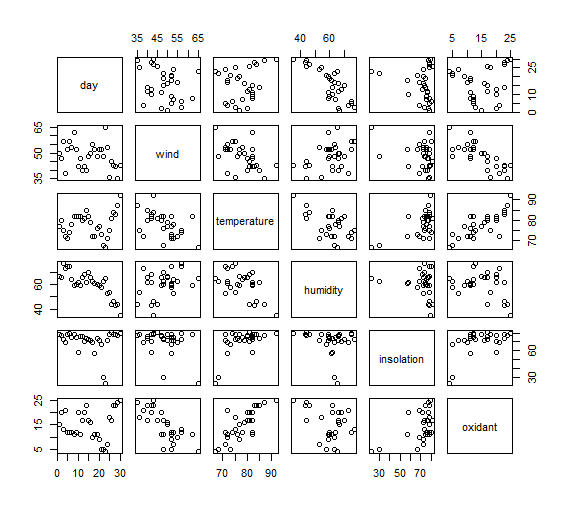
\includegraphics[scale=0.6]{../results/2_1.png}
          \caption{Pairplot of the airpollution data}
          \label{fig:BoxHours}
      \end{figure} 
    \subsection*{2}
      \begin{figure}[H]
          \centering
          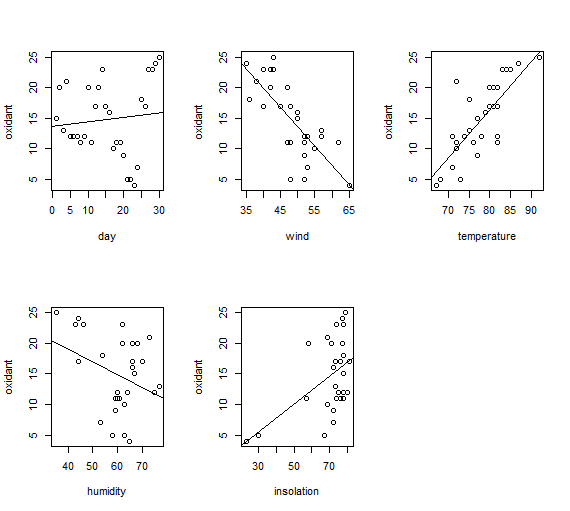
\includegraphics[scale=0.6]{../results/2_2.png}
          \caption{The linear regression of the explanatory variables}
          \label{fig:BoxHours}
      \end{figure} 
    \subsection*{3}
    \subsection*{4}
    \subsection*{5}

  \section*{Exercise 3}
    \subsection*{1}
    \subsection*{2}
    \subsection*{3}
    \subsection*{4}
    \subsection*{5}

  \section*{Exercise 4}
    The dataset \textit{expensescrime} is exolored.
    The response variable is \textit{expend} and the rest are independent variables.
    In Fig\ref{fig:PairsCrime} the pairs plot of the data is shown.
    There you can see some correlation between the response variable and the rest,
    namely between expend and every variable except crime.
    This is researched further by looking at the correlation matrix Table\ref{table:cormatrix}, also shown in Fig\ref{table:cormatrix}.
    \begin{table}[H]
    \begin{center}
    \begin{tabular}{l|llllll}
             & bad & crime & lawyers & employ & pop &expend \\
      \hline
      bad    & 1.00 & 0.37 & 0.83 & 0.87 & 0.92 & 0.83 \\
      crime  & 0.37 & 1.00 & 0.38 & 0.31 & 0.28 & 0.33 \\
      lawyers& 0.83 & 0.38 & 1.00 & 0.97 & 0.93 & 0.97 \\
      employ & 0.87 & 0.31 & 0.97 & 1.00 & 0.97 & 0.98 \\
      pop    & 0.92 & 0.28 & 0.93 & 0.97 & 1.00 & 0.95 \\
      expend & 0.83 & 0.33 & 0.97 & 0.98 & 0.95 & 1.00 \\
    \end{tabular}
    \caption{Correlation matrix}
    \label{table:cormatrix}
    \end{center}
    \end{table}

    \begin{figure}[H]
        \centering
        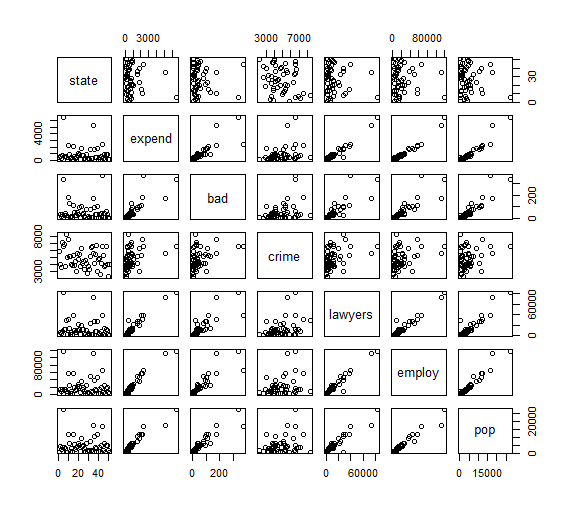
\includegraphics[scale=0.4]{../results/4_pairs.png}
        \caption{The pairs plot}
        \label{fig:PairsCrime}
    \end{figure} 

    \begin{figure}
        \centering
        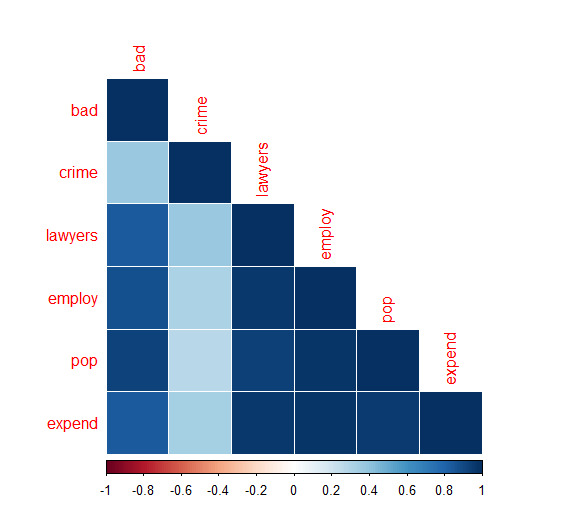
\includegraphics[scale=0.4]{../results/4_lower_corrplot.png}
        \caption{The correlation plot}
        \label{fig:cormatrix}
    \end{figure} 

    To be able to find the linear regression model of this data two methods can be used.
    The step-up and the step-down method.
    Following the step-up method we get the steps found in Table\ref{table:step-up}:
    \begin{table}
    \begin{center}
    \begin{tabular}{|ll|}
        \hline
        Variable & $R^2$ \\
        \hline 
        Step1&\\
        \hline
        Expend\textasciitilde Pop & 0.9073 \\
        Expend\textasciitilde Employ & 0.954 \\
        Expend\textasciitilde Lawyers & 0.9373 \\
        Expend\textasciitilde Crime & 0.1119 \\
        Expend\textasciitilde Bad & 0.6964 \\
        \hline
        Step2&\\
        \hline 
        Expend\textasciitilde Employ+Pop & 0.9543 \\
        Expend\textasciitilde Employ+Lawyers & 0.9632 \\
        Expend\textasciitilde Employ+Crime & 0.9551 \\
        Expend\textasciitilde Employ+Bad & 0.9551 \\
        \hline
        Step3&\\
        \hline 
        Expend\textasciitilde Employ+Lawyers+Pop & 0.9637 \\
        Expend\textasciitilde Employ+Lawyers+Crime & 0.9632 \\
        Expend\textasciitilde Employ+Lawyers+Bad & 0.9639 \\
        \hline
    \end{tabular}
    \caption{Step-up method}
    \label{table:step-up}
    \end{center}
    \end{table}
    \begin{table}
    \begin{center}
    \begin{tabular}{|ll|}
        \hline
        Variable & \textit{p} \\
        \hline 
        Step1&\\
        \hline
        Expend\textasciitilde Employ+Lawyers+Bad+Pop+Crime & $R^2 = 0.9666$ \\
        Employ & 0.00354 \\
        Lawyers & 0.00592 \\
        Bad & 0.02719 \\
        Pop & 0.03184 \\
        Crime & 0.25534\\
        \hline
        Step2&\\
        \hline 
        Expend\textasciitilde Employ+Lawyers+Bad+Pop & $R^2 = 0.9666$ \\
        Employ & 0.00380 \\
        Lawyers & 0.00106 \\
        Bad & 0.05402 \\
        Pop & 0.06012 \\
        \hline
        Step3&\\
        \hline 
        Expend\textasciitilde Employ+Lawyers+Bad & $R^2 = 0.9666$ \\
        Employ & 1.2e-06 \\
        Lawyers & 0.00147 \\
        Bad & 0.34496 \\
        \hline
        Step4&\\
        \hline 
        Expend\textasciitilde Employ+Lawyers+Bad & $R^2 = 0.9666$ \\0.00113
        Employ & 4.89e-07 \\
        Lawyers & 0.00113 \\
        \hline
    \end{tabular}
    \caption{Step-down method}
    \label{table:step-down}
    \end{center}
    \end{table}
    Both methods end up with the same formula, namely Expend\textasciitilde Employ+Lawyer.
    The results of this is:
    \begin{lstlisting}[language=R]
Coefficients:
              Estimate Std. Error t value Pr(>|t|)    
(Intercept) -1.107e+02  4.257e+01  -2.600  0.01236 *  
employ       2.971e-02  5.114e-03   5.810 4.89e-07 ***
lawyers      2.686e-02  7.757e-03   3.463  0.00113 ** 
Multiple R-squared:  0.9632
    \end{lstlisting}
    Which means that the formula for Expend is as follows:
    \[
      Expend = -1.107e^2 + 2.971e^{-2} * Employ + 2.686e^{-2} * Lawyers.
    \]
    \\

    Researching if this is a good result includes looking for influence points, collinearity and residuals.
    The influence points can be found by cook's distance, seen in Fig\ref{fig:4cook}.
    There are only two significant datapoints that can influence the methods used.
    \begin{figure}
        \centering
        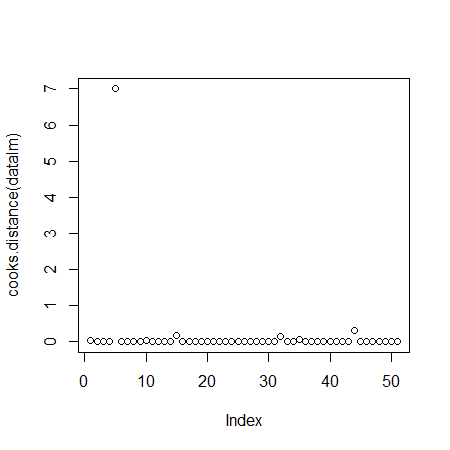
\includegraphics[scale=0.4]{../results/4_cook.png}
        \caption{The cook's distance}
        \label{fig:4cook}
    \end{figure}
    The Collinearity can be seen by looking at the Fig\ref{fig:cormatrix} and Table\ref{table:cormatrix}, here you see that 
    most of the variables have a sort of correlation with each other.
    The residuals can be found in Fig\ref{fig:4res}, which indicate that the data is not linearly correlated.
    None of the data in the plots is randomly scattered.
    This is backed up by Fig\ref{fig:4qq}
    \begin{figure}
        \centering
        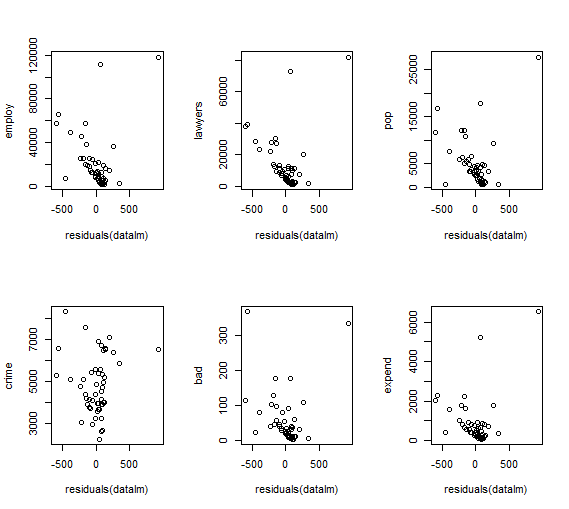
\includegraphics[scale=0.4]{../results/4_res.png}
        \caption{The residuals of the regression}
        \label{fig:4res}
    \end{figure}
    \begin{figure}
        \centering
        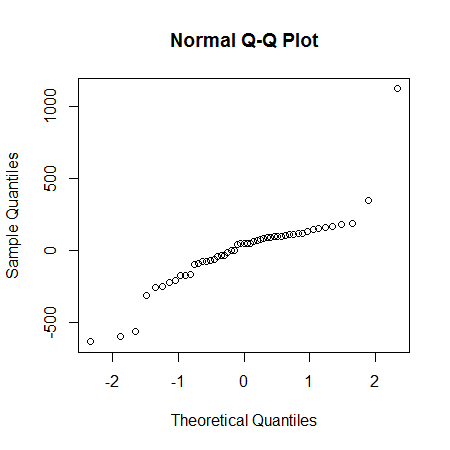
\includegraphics[scale=0.4]{../results/4_qq.png}
        \caption{QQ-plot of the residuals}
        \label{fig:4qq}
    \end{figure}
    
  \section{R-Code}
    \subsection{Exercise 1}\label{sec:RE1}
      \begin{lstlisting}[language=R]
      \end{lstlisting}
    \subsection{Exercise 2}\label{sec:RE2}
      \begin{lstlisting}[language=R]
      \end{lstlisting}
    \subsection{Exercise 3}\label{sec:RE3}
      \begin{lstlisting}[language=R]
      \end{lstlisting}
    \subsection{Exercise 4}\label{sec:RE4}
      \begin{lstlisting}[language=R]
      \end{lstlisting}
\end{document}
